%%%%%%%%%%%%%%%%%%%%%%%%%%%%% Define Article %%%%%%%%%%%%%%%%%%%%%%%%%%%%%%%%%%
\documentclass{article}
%%%%%%%%%%%%%%%%%%%%%%%%%%%%%%%%%%%%%%%%%%%%%%%%%%%%%%%%%%%%%%%%%%%%%%%%%%%%%%%

%%%%%%%%%%%%%%%%%%%%%%%%%%%%% Using Packages %%%%%%%%%%%%%%%%%%%%%%%%%%%%%%%%%%
\usepackage{geometry}
\usepackage{graphicx}
\usepackage{amssymb}
\usepackage{amsmath}
\usepackage{amsthm}
\usepackage{empheq}
\usepackage{mdframed}
\usepackage{booktabs}
\usepackage{lipsum}
\usepackage{graphicx}
\usepackage{color}
\usepackage{psfrag}
\usepackage{pgfplots}
\usepackage{bm}
%%%%%%%%%%%%%%%%%%%%%%%%%%%%%%%%%%%%%%%%%%%%%%%%%%%%%%%%%%%%%%%%%%%%%%%%%%%%%%%

% Other Settings

%%%%%%%%%%%%%%%%%%%%%%%%%% Page Setting %%%%%%%%%%%%%%%%%%%%%%%%%%%%%%%%%%%%%%%
\geometry{a4paper}

%%%%%%%%%%%%%%%%%%%%%%%%%% Define some useful colors %%%%%%%%%%%%%%%%%%%%%%%%%%
\definecolor{ocre}{RGB}{243,102,25}
\definecolor{mygray}{RGB}{243,243,244}
\definecolor{deepGreen}{RGB}{26,111,0}
\definecolor{shallowGreen}{RGB}{235,255,255}
\definecolor{deepBlue}{RGB}{61,124,222}
\definecolor{shallowBlue}{RGB}{235,249,255}
%%%%%%%%%%%%%%%%%%%%%%%%%%%%%%%%%%%%%%%%%%%%%%%%%%%%%%%%%%%%%%%%%%%%%%%%%%%%%%%

%%%%%%%%%%%%%%%%%%%%%%%%%% Define an orangebox command %%%%%%%%%%%%%%%%%%%%%%%%
\newcommand\orangebox[1]{\fcolorbox{ocre}{mygray}{\hspace{1em}#1\hspace{1em}}}
%%%%%%%%%%%%%%%%%%%%%%%%%%%%%%%%%%%%%%%%%%%%%%%%%%%%%%%%%%%%%%%%%%%%%%%%%%%%%%%

%%%%%%%%%%%%%%%%%%%%%%%%%%%% English Environments %%%%%%%%%%%%%%%%%%%%%%%%%%%%%
\newtheoremstyle{mytheoremstyle}{3pt}{3pt}{\normalfont}{0cm}{\rmfamily\bfseries}{}{1em}{{\color{black}\thmname{#1}~\thmnumber{#2}}\thmnote{\,--\,#3}}
\newtheoremstyle{myproblemstyle}{3pt}{3pt}{\normalfont}{0cm}{\rmfamily\bfseries}{}{1em}{{\color{black}\thmname{#1}~\thmnumber{#2}}\thmnote{\,--\,#3}}
\theoremstyle{mytheoremstyle}
\newmdtheoremenv[linewidth=1pt,backgroundcolor=shallowGreen,linecolor=deepGreen,leftmargin=0pt,innerleftmargin=20pt,innerrightmargin=20pt,]{theorem}{Theorem}[section]
\theoremstyle{mytheoremstyle}
\newmdtheoremenv[linewidth=1pt,backgroundcolor=shallowBlue,linecolor=deepBlue,leftmargin=0pt,innerleftmargin=20pt,innerrightmargin=20pt,]{definition}{Definition}[section]
\theoremstyle{myproblemstyle}
\newmdtheoremenv[linecolor=black,leftmargin=0pt,innerleftmargin=10pt,innerrightmargin=10pt,]{problem}{Problem}[section]
\theoremstyle{myproblemstyle}
\newmdtheoremenv[linecolor=black,leftmargin=0pt,innerleftmargin=10pt,innerrightmargin=10pt,]{example}{Example}[section]
\parindent=0pt
\parskip=3pt
%%%%%%%%%%%%%%%%%%%%%%%%%%%%%%%%%%%%%%%%%%%%%%%%%%%%%%%%%%%%%%%%%%%%%%%%%%%%%%%

%%%%%%%%%%%%%%%%%%%%%%%%%%%%%%% Plotting Settings %%%%%%%%%%%%%%%%%%%%%%%%%%%%%
\usepgfplotslibrary{colorbrewer}
\pgfplotsset{width=8cm,compat=1.9}
%%%%%%%%%%%%%%%%%%%%%%%%%%%%%%%%%%%%%%%%%%%%%%%%%%%%%%%%%%%%%%%%%%%%%%%%%%%%%%%

%%%%%%%%%%%%%%%%%%%%%%%%%%%%%%% Title & Author %%%%%%%%%%%%%%%%%%%%%%%%%%%%%%%%
\title{Problem Solving Strategies}
\author{Alston Yam}
%%%%%%%%%%%%%%%%%%%%%%%%%%%%%%%%%%%%%%%%%%%%%%%%%%%%%%%%%%%%%%%%%%%%%%%%%%%%%%%

\begin{document}
    \maketitle

    \section{Make an ORGANISED List}
    Here, we are basically listing out all the possible answers to a question. However, it is \textbf{VERY IMPORTANT} that you list it with some order, so you don't get lost.

    \begin{example}
        Tanya and Mona are in the Big Beast Booth at the country fair. Tanya buys a ticket which gives her three throws with a bean bag at the bears. There are four bears, each with a different number on it: 1, 2, 3 and 4. Each time Tanya hits a bear she gets the number of points printed on the bear. After three throws the points are added up and she gets a prize for any score over zero. Tanya's score is 4. How many different ways could Tanya have scored 4 points?
    \end{example}

    \textit{ Sol. }We can first list out in how many ways can Tanya get 4 points. We can list them out in order like so: 004, 013, 022, 112. Notice that I'm listing them, starting if the first throw was 0, then moving to if the first throw is 1. 

    Are we done?

    No. We need to consider the order in which the points are scored: 004 can also be 040, or 400. We can list all the values out like this:

    \begin{align*}
        004 &: 004, 040, 400\\
        013 &: 013, 031, 103, 130, 301, 310\\
        022 &: 022, 202, 220 \\
        112 &: 112, 121, 211
    \end{align*}

    Now we count, and we see a total of 15 ways.

    \begin{problem}
        In the movie "Moon Monster" the hero has to win a game of darts in order to escape from the Tiny Tidbits. The balloon-dart game has 3 balloons taped to a board. The balloons are marked 10, 20 and 30 points. The player gets three darts or three tries to score as many points as possible. The Tiny Tidbits are not too good at this game, so the hero wins with a score of 30 points. How many different ways ($0+0+30$ is different from $0+30+0$) could the hero have scored 30 points? 
    \end{problem}

    \begin{problem}
        James spent 1 dollar at a store, and got change for 36 cents. If the following coin denominations are available: 1 cent, 5 cent, 10 cent and 25 cent, What are the possible combinations of coins that James could have received for his change of 36 cents?
    \end{problem}

     \section{Make a table}
    We are going to make a table, to keep track of some information in the question.

    \begin{example}
        Plans are underway for the New Zealand Police local Olympics. Among the participants will be representatives from the three least densely populated districts in NZ. For every 8 athletes from Tasman, there will be 12 athletes from Southland and 9 from Northland. How many representatives will there be altogether from these three districts, if 72 athletes are expected from Northland?
    \end{example}

    \begin{center}
        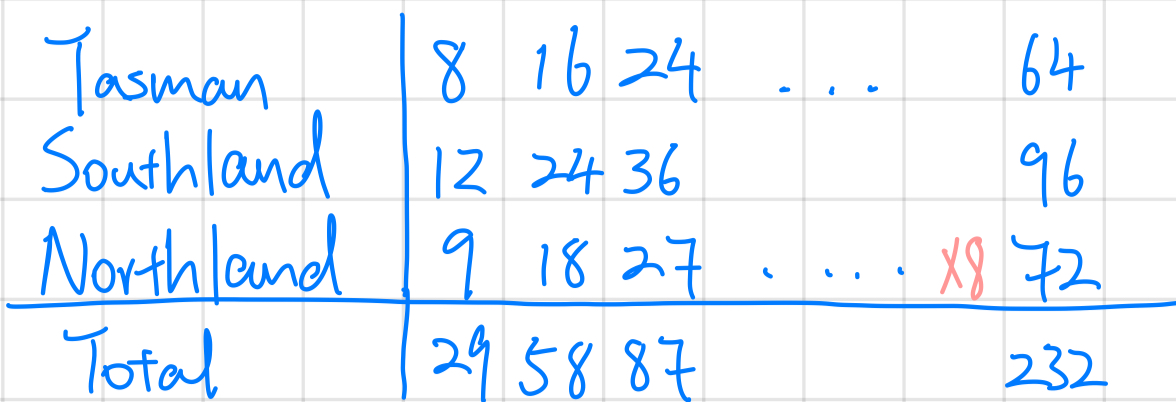
\includegraphics[width=0.8\textwidth]{makeatable.jpeg}
    \end{center}

    So we can see that the answer is 232 athletes.

    \begin{problem}
        Ann and Makiko like to swim laps at the local pool. They are swimming together today, but they are on different swim schedules. Ann swims every three days and Makiko swims every five days. How many times will they both be in the pool on the same day in the next ten weeks?
    \end{problem}

    \begin{problem}
        It is 12:00 and people are lining up for the matinee at the Bijou Cinema Six. In the first five minutes (12:05) 6 people got into the line. At the end of the second five minutes (12:10) there were 11 people in the line. At the end of the third five minutes (12:15), there are 16 people in the line. If the people keep lining up at the same rate, what time will it be when there are 81 people in the line?
    \end{problem}

    \section{Using patterns}
    Try out the first few small numbers. Can you spot any patterns that will be useful for other, bigger values too?

    There are mainly 3 types of patterns:

    \begin{theorem}[differences]
        If the numbers add by a specific number.
        \[1, 3, 5, 7, 9, \cdots \]
        Here we have the numbers adding 2 each time.
    \end{theorem}

    \begin{theorem}[ratio]
        \[1, 2, 4, 8, 16, 32, \cdots\]

        We are multiplying by 2 to get the next number.
    \end{theorem}

    \begin{theorem}[special sequences]
        \[1, 4, 9, 16, 25, \cdots\]
        \[1, 8, 27, 64, 125, \cdots\]
        \[1, 1, 2, 3, 5, 8, 13, 21, \cdots\]
        \[1, 3, 6, 10, 15, 21, \cdots\]

        What are each of these sequeces? You need to remember the first few numbers of these sequences.
    \end{theorem}

    \begin{example}
        In a country, towns are set up in an interesting way. First town had 1 house, second town had 3 houses, third town has 6 houses, and so on. Each town is formed in a triangular shape of houses. How many houses would be in town nine?
    \end{example}

    \textit{ Sol. } If we imagine the houses in each town, we see that there are 1, 3, 6, 10, 15 $\cdots$ houses. This is actually a sequence called the Triangular Numbers, and the pattern has that we are doing +1, +2, +3 ... to get the next number. If we list it out, we can see that town nine will have 45 houses.

    \begin{problem}
        In the mountains, people are saying that they are seeing Bigfoot. The first day, 6 people called the police. The next day, twice as many people called the police, compared to the previous day. On what day did the police receive their 300th call?
    \end{problem}

    \section{Working backwards}
    Start from the answer of the question, and trace back your steps.

    \textbf{This is the easiest way to check your answer!}

    \begin{example}
        Kevin, Barbara and their mother and father went tramping in a park. On the first and second day each hiker had a serving of food for breakfast, lunch and dinner. On the second night, a large noisy brown bear barged into their camp and got the food pack down from the tree where they had hung it, and ate one half of the food that was left. The next morning, after they had all eaten breakfast, they found they had 4 servings of food left. How many servings of food did they begin the trip with?
    \end{example}

    \textit{ Sol. } Lets backtrack in time. On the last day, they each ate one serving of food for breakfast, so they ate a total of 4 servings. This means that before they had breakfast, they had 8 servings of food in total. (this is because we know that there had been 4 servings left over at the end).

    Now, these 8 servings are what's left, after the bear had ate some. The bear ate exactly half of the food, and left 8. This means that the 8 left was half of what was there originally, so before the bear ate anything, there had been $8 \times 2 = 16$ servings of food.

    Now we just need to look back to the first 2 days. Each person ate 3 servings of food each day, and there are 4 people. So each day, a total of 12 servings of food are eaten. This happened for the first 2 days. So they ate $12 + 12 = 24$ servings in total.

    So we must know that they started off with $16 + 24 = 40$ servings of food.

    \begin{example}
        Bob the builder is building a house. Throughout the day, He used 7 pieces of wood for the door, two thirds of what's remaining on the walls, he then got a delivery of 10 pieces of wood, and spent half of what he has on the windows. He is left with 7 pieces of wood. How many pieces of wood did he have at the start of the day?
    \end{example}
    
    
    \section{Simplifying the problem}
    When a problem is complicated, can you break down the problem to several parts that you can solve one at a time?

    \begin{example}
        A group of 13 friends were planning a trip. On the night before they left, they made a lot of phone calls. Each friend talked to every other friend at least once. What is the fewest number of phone calls that could have been made?
    \end{example}

    \textit{ Sol. } Wait... so it's really hard to think about 13 friends all at once. So why don't we think about something easier: if we got 2 friends only. Well then, we only need 1 call right?

    Now if we have 3 friends. We can try it out, and see that we only need 3 calls. 

    If we have 4 friends, we can see that at the fewest, we need 6 calls.

    If you are keen eyed, then you should be able to see that this is just the triangular numbers! So working upwards all the way to 13 friends, we can find out how many calls we need.
   
    \begin{problem}
        Your sock drawer has 25 yellow socks, 30 blue socks, 17 orange socks, 13 magenta socks, 33 purple socks, 30 red socks, 11 green socks, 14 black socks and 23 brown socks. If you reach into the drawer in the dark, how many socks do you need to pull out to be sure you have a matching pair?
    \end{problem}


    \section{Use a diagram}
    Draw out the diagram to visualise the problem, then \textbf{USE} your diagram to figure out the question.

    \begin{example}
        Sandy is delivering pizza to the second floor of an apartment. There are two outside stairways from the street to the building. Then there are four doors into the building. Once inside there are two elevators and two inside stairways that go to the second floor. How many different ways can Sandy go from the street to the second floor and deliver the pizza?
    \end{example}

    \begin{center}
        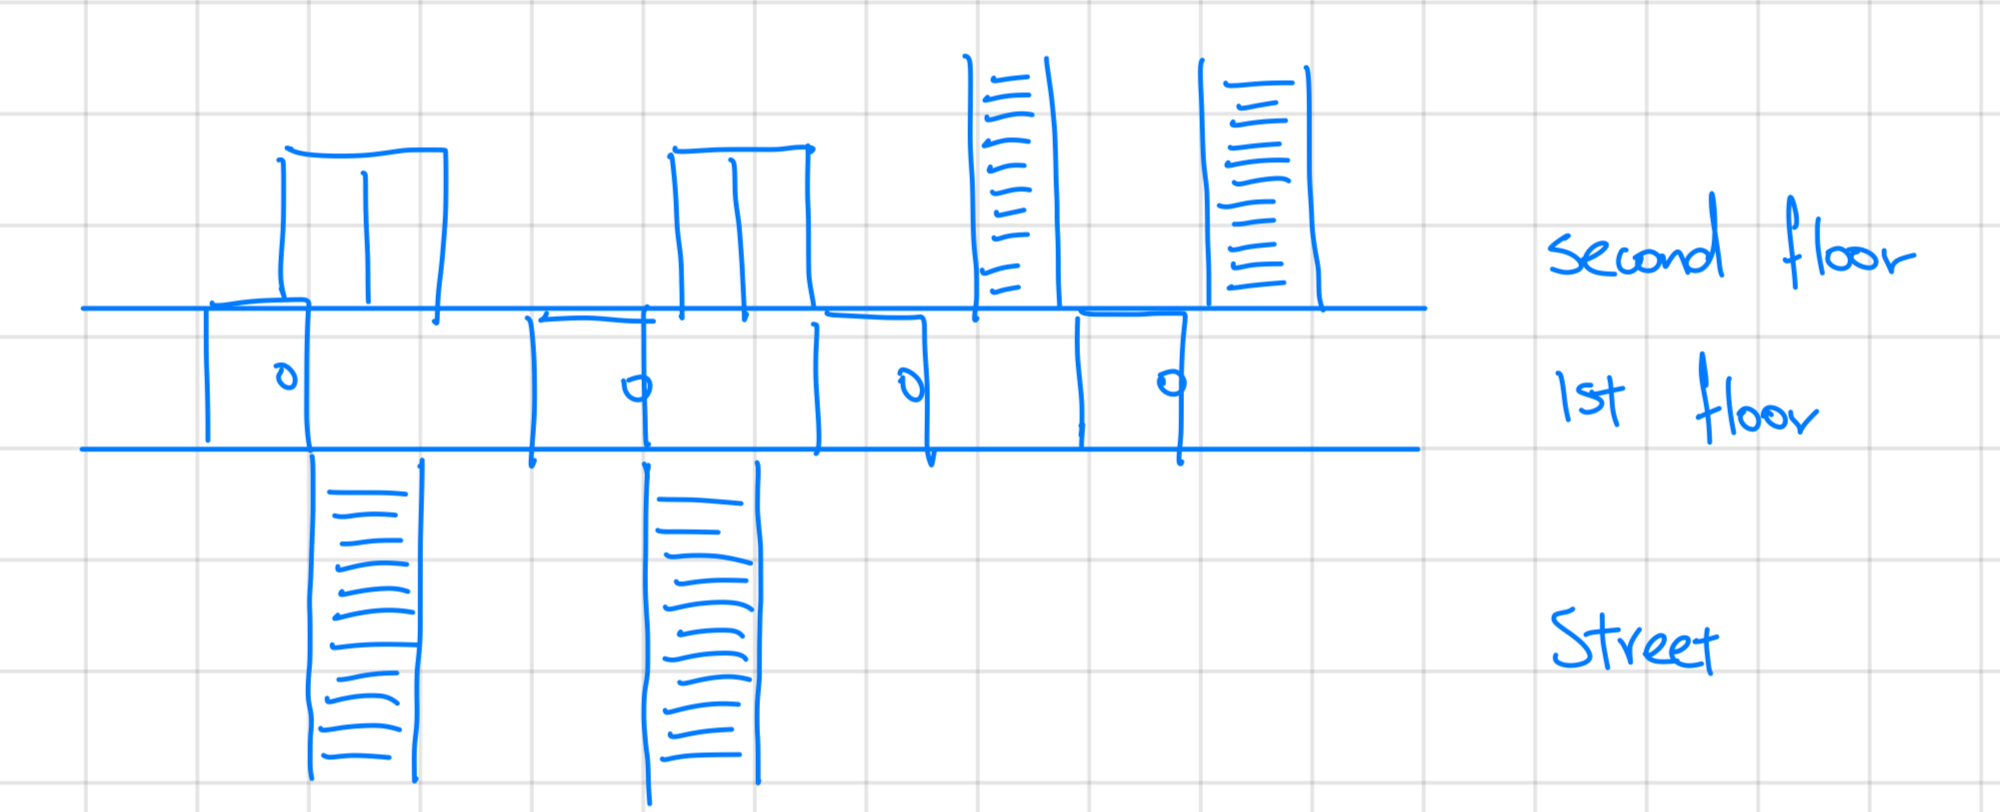
\includegraphics[width=0.8\textwidth]{Diagram.jpeg}
    \end{center}

    We now see we have $2 \times 4 \times 4 = 32$ ways... very straight forward to count!

    \begin{problem}
        Sara's softball team can be divided into four groups: $\frac{1}{2}$ of the group are hitters, $\frac{1}{4}$ are good pitchers, $\frac{1}{8}$ like to play outfield and 2 players are catchers. If each player is only in one group, how many players are on the team, and how many players are in each group?
    \end{problem}

    \section{Act it out}
    Follow the logic of the question.

    \begin{problem}
        Andre's Blue Ribbon Car and Trucks is having a big sale. Mike and Don are setting up the lot. The boss gives them a diagram of the lot and these directions: "Put the 4-door car in front of the van. Put the jeep between the truck and the van. Put the sports car to the left of the 2-door and 4-door cars." How did Mike and Don set up the lot?
    \end{problem}

    \begin{problem}
        Armando has a card trick for Andrew: "I have 10 cards, numbered from 1 to 10. I have arranged the cards in a stack in a special way. The first card facing up is a 1, and I'm putting it on the table. The second card I'm putting at the bottom of the stack. The third card, which is a 2, I'm putting on the table next to the 1. Then the fourth card goes to the bottom of the stack. I'll continue putting one card on the table and the next one on the bottom of the stack until I put card 10 on the table. How do I first arrange the cards in a stack?"
    \end{problem}


\end{document}